\documentclass{scrreprt}
\usepackage[dutch]{babel}
\usepackage{graphicx}
\usepackage{etoolbox}
\usepackage{float}

%Remove newpage from chapter
\makeatletter
\patchcmd{\scr@startchapter}{\if@openright\cleardoublepage\else\clearpage\fi}{}{}{}
\makeatother
\DeclareGraphicsExtensions{.pdf,.png,.jpg}

\title{Software Wijziging Proces}
\author{Guus Hamm en Rick Rongen}
\date{\today}

\begin{document}
	\maketitle
	\tableofcontents
	\newpage
	\chapter{Software Wijzigings Proces}
		Zodra ons product in productie staat, kan het niet zomaar meer gewijzigd worden. Hierom is het belangrijk dat er een duidelijk proces wordt vastgezet voor het accepteren en aanbrengen van wijzigingen.
	
	\chapter{Acceptatie}
	\begin{figure}[ht]
		\centering
		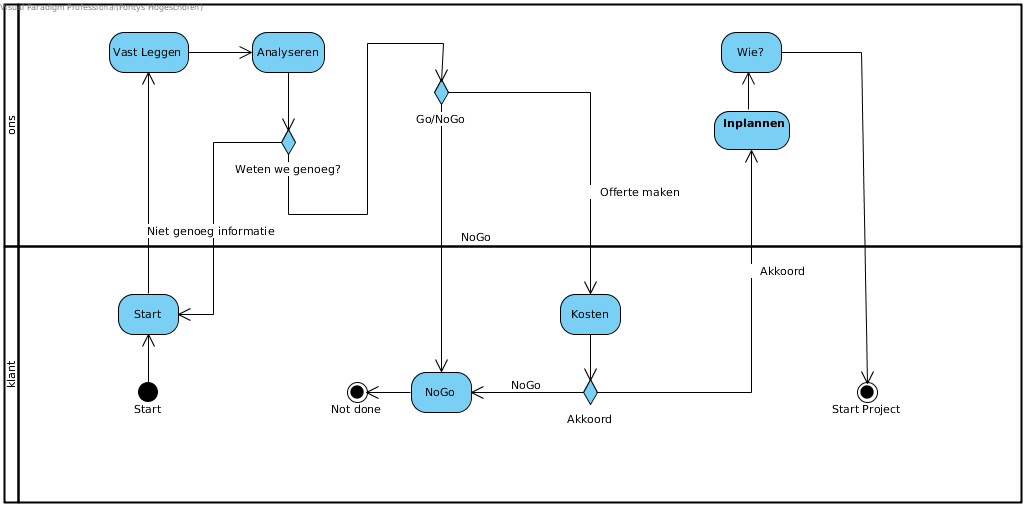
\includegraphics[width=\linewidth]{change-request}
		\label{fig:change-request}
		\caption{Change Request}
	\end{figure}
		Als er een wijzigings aanvraag van binnen of buiten af aankomt, dan wordt dit proces opgestart om te bepalen of en wanneer de wijziging wordt toegepast.\par
		
		Als eerste wordt het probleem vastgelegd en onderzocht. Hierna wordt bepaald of er genoeg informatie beschikbaar is, zo niet dan wordt dit teruggekoppeld aan de aanvrager.\par
		Als er voldoende informatie beschikbaar is, dan wordt er een GO of NOGO gegeven. Als het niet waard of niet mogelijk is om de wijziging toe te voegen, dan wordt dit nu terug gekoppeld aan de klant.\par
		Hierna wordt er kosten vastgesteld voor de wijziging. Deze kosten omvatten onder meer de uren die er aan gespendeerd moeten worden, het testen en het uitbrengen en ondersteunen. Deze kosten worden gepresenteerd aan de klant, die hierop een keuze kan maken om door te gaan met het proces of er toch mee te stoppen.\par
		Als laatste wordt er gepland wanneer de feature wordt gemaakt en wie dit gaat doen. Als dit allemaal bekend is dan kan het project voor de wijziging gestart worden.
	\chapter{Implementatie en Testen}
		\begin{figure}[ht]
			\centering
			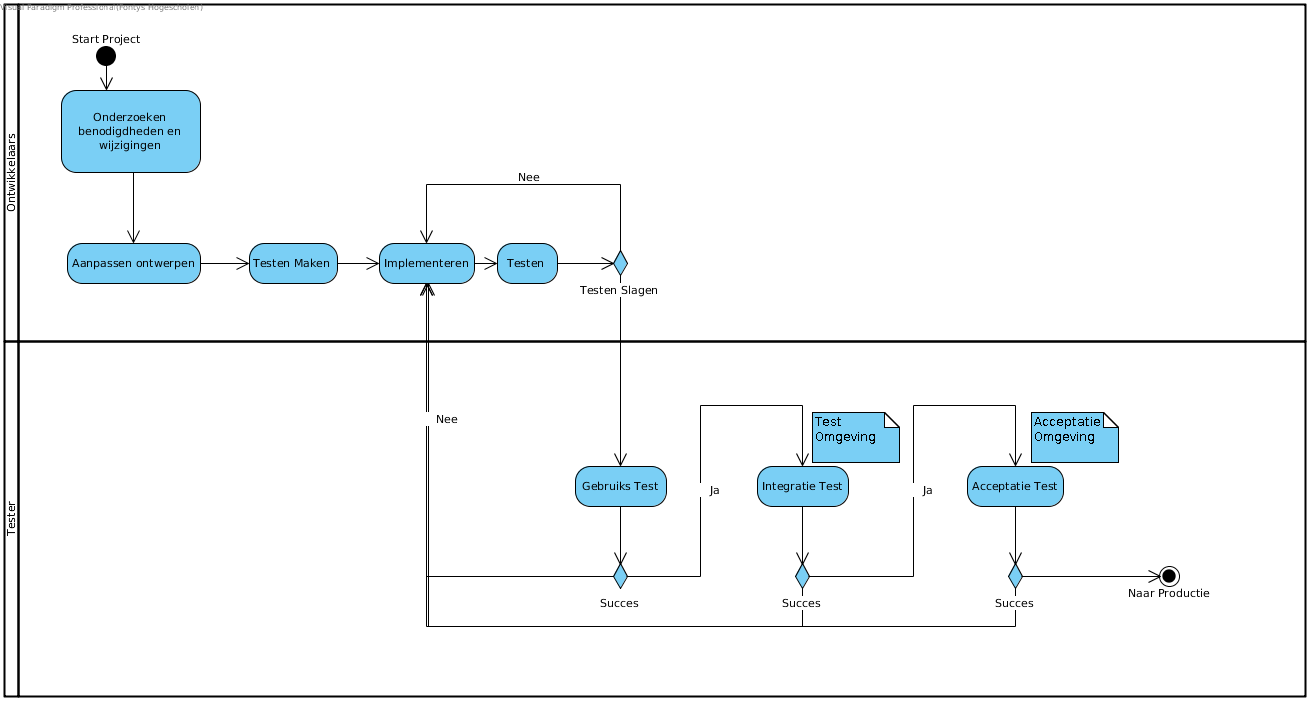
\includegraphics[width=\linewidth]{implementation-testing}
			\label{fig:implementation-testing}
			\caption{Implementatie en Testen}
		\end{figure}
		In het begin van dit proces wordt er eerst onderzocht wat er precies gewijzigd moet worden en wat daar voor nodig is. Denk aan bibliotheken, nieuwe componenten en het wijzigingen van code.\par
		Als dit onderzocht is worden deze wijzigingen in de ontwerpen van de applicatie verwerkt. Zodat iedere ontwikkelaar kan zien hoe het er (globaal) uit moet gaan zien.\par
		Nadat het ontwerp af is worden er unit tests geschreven om de nieuwe code af te testen. Deze test waarborgen dan het resultaat ook het verwachte resultaat is.\par
		Hierna wordt er een Implementatie en Test cyclus gestart. Nadat een onderdeel gemaakt is, dan wordt deze getest. Zodra alle onderdelen geïmplementeerd zijn, de unit tests slagen en de ontwikkelaars en zeker van zijn dat de code goed is. Dan wordt het project doorgezet om afgetest te worden.\par
		\section{Testen}
		De tester doorlopen 3 test fases, waar na iedere fase het project terug gezet kan worden naar implementatie als het niet goed is.\par
		Als eerste wordt er getest of het product nog goed bruikbaar is na de wijzigingen, kan alles nog bereikt worden, zijn de nieuwe onderdelen intuïtief, werkt het überhaupt.\par
		Als deze test geslaagd is, dan word het product getest in de test omgeving. Hier word getest of het goed samenwerkt met de andere producten in de omgeving en geen problemen veroorzaakt.\par
		De laatste test zal kijken of het product ook goed blijft werken als het op een productie omgeving staat. Deze test loopt op de integratie omgeving, die vrijwel identiek is aan de productie omgeving. Hier kan ook getest worden of het product de productie lading kan weerstaan en of het met alles kan blijven samenwerken.
\end{document}